\PassOptionsToPackage{table}{xcolor}
\documentclass[10pt]{beamer}
\usepackage[english]{babel}

\usetheme{metropolis}
\usepackage{smartdiagram}
\usepackage{listings}
\usepackage{booktabs}
\usepackage[scale=2]{ccicons}%creative commons
\setbeamercovered{transparent}%invisible by default
\usepackage{array}
\newcolumntype{L}[1]{>{\raggedright\let\newline\\\arraybackslash\hspace{0pt}}m{#1}}
\newcolumntype{C}[1]{>{\centering\let\newline\\\arraybackslash\hspace{0pt}}m{#1}}
\newcolumntype{R}[1]{>{\raggedleft\let\newline\\\arraybackslash\hspace{0pt}}m{#1}}

\usepackage{pgfplots}
\usepgfplotslibrary{dateplot}
\usepackage{tikz}
\usepackage{tikz-uml}
\usetikzlibrary{positioning,chains,fit,shapes,calc}

\newcommand{\mycomment}[1]{}
\usepackage{fancyvrb}
% *****************************************************************************
% Matematica 
% *****************************************************************************

%\usepackage{amssymb}
%\usepackage{mathtools}                    % Add support for cramped,
					  
%\usepackage[euler]{flexisym}
%\usepackage{breqn}                        % Breqn
%\makeatletter
%   \def\eqnumsize{\normalfont \Tf@font}      % Add support to Minion Pro
%\makeatother
%\setkeys{breqn}{labelprefix={eq:}}


%\usepackage{asymptote}
%\usepackage[loop, controls]{animate}

\graphicspath{{./}, {./Images/}}

\lstdefinelanguage{Kotlin}{
  keywords={package, as, typealias, this, super, val, var, fun, for, null, true, false, is, in, throw, return, break, continue, object, if, try, else, while, do, when, yield, typeof, yield, typeof, class, interface, enum, object, override, public, private, get, set, import, abstract, },
  keywordstyle=\color{blue}\bfseries,
  ndkeywords={@Deprecated, Int, Integer, Float, Double, String, Runnable, dynamic},
  ndkeywordstyle=\color{red}\bfseries,
  emph={println, return@, forEach,},
  emphstyle={\color{red}},
  identifierstyle=\color{black},
  sensitive=true,
  commentstyle=\color{gray}\ttfamily,
  comment=[l]{//},
  morecomment=[s]{/*}{*/},
  stringstyle=\color{gray}\ttfamily,
  morestring=[b]",
  morestring=[s]{"""*}{*"""},
}

\providecommand{\ie}{i.\,e.}
\providecommand{\Ie}{I.\,e.}
\providecommand{\eg}{e.\,g.}
\providecommand{\Eg}{E.\,g.} 

\metroset{block=fill}
\metroset{titleformat frame=smallcaps}

\title{Dependency injection made easy with Dagger2}
%\subtitle{and how it can help us building better reactive code}

\date{\today}
\author[A. Candolini]{Alessandro Candolini}
%\institute{Department of Physics, University of Trieste}
% \titlegraphic{\hfill\includegraphics[height=1.5cm]{logo/logo}}

\begin{document}

\maketitle

\begin{frame}{Agenda}
  \setbeamertemplate{section in toc}[sections numbered]
  \tableofcontents[hideallsubsections]
\end{frame}

\section{Dependency injection principles}
\begin{frame}[fragile]
	\frametitle{What is a dependency?}
		\begin{figure}
			\centering
\begin{tikzpicture}
\umlsimpleclass [minimum height=15ex,width=15ex] {A}
	\umlsimpleclass[x=4,width=5ex]{B}
\umlunicompo[geometry=|-|]{A}{B}
\end{tikzpicture}
		\end{figure}
\end{frame}
\begin{frame}[fragile]
%\begin{lstlisting}[language=java,basicstyle=\ttfamily,keywordstyle=\color{red}]
\begin{lstlisting}[language=Kotlin, basicstyle=\ttfamily]
/** Class A (the client) */
class A {
    // ....
    fun doSomething() {
        b.log("text")
    }
}

/** Class B (dependency/service) */
class B {
    fun log(text : String) {
    }
}
\end{lstlisting} 
\end{frame}
	\begin{frame}[fragile]
\begin{lstlisting}[language=Kotlin, basicstyle=\ttfamily]
// Option 1 - static methods 

class A {
    fun doSomething() {
        B.log("text") // <- static method
    }
}

class B {
    companion object {
        fun log(text: String) {
        }
    }
}
\end{lstlisting} 
	\end{frame}

	\begin{frame}
		Examples:
		\begin{itemize}
			\item Helper  classes
			\item Utils  classes
			\item Manager classes, etc\ldots
		\end{itemize}
	\end{frame}

	\begin{frame}[fragile]
		Drawbacks:
		\begin{itemize}
			\item $A$ not testable in isolation (integration test of $A$ \& $B$)
			\item $A$ \emph{strongly coupled} to $B$ (hardcoded dependency, no way to override/replace it) 
			\item Lack of encapsulation  (backdoor) 
			\item \emph{Hidden} dependency 
		\end{itemize}
	\end{frame}
	\begin{frame}[fragile]
		More Examples:
		\begin{itemize}
			\item \verb|Application.getStaticContext()|
			\item in order to move one class to a different module, you have to move ``hundreds`` of classes\ldots 
		\end{itemize}
	\end{frame}
\begin{frame}[fragile]
\begin{lstlisting}[language=Kotlin, basicstyle=\ttfamily]
// Option 2 - singletons

class A {
    fun doSomething() {
	B.log("text") // <- singleton
    }
}

object B {
    fun log(text: String) {
    }
}
\end{lstlisting} 
\end{frame}
\begin{frame}[fragile]
\begin{lstlisting}[language=Kotlin, basicstyle=\ttfamily]
// Option 3 - composition 

class A {
    private val b : B = B() // <-- instantiate
    
    fun doSomething() {
        b.log("text")
    }
}

class B {
    fun log(text: String) {
    }
}
\end{lstlisting} 
\end{frame}
	\begin{frame}[fragile]
		%\frametitle{Composition}
		\begin{figure}
			\centering
\begin{tikzpicture}
	\umlclass{A}{}{+ doSomething() : void}
	\umlclass [x=5, y=0] {B}{}{+ log(text : String) : void}
\umlunicompo{A}{B}
\end{tikzpicture}
		\end{figure}
			The \emph{life} of the child is completely controlled by the parent.
%\begin{tikzpicture}
%\umlsimpleclass [x=0,width=15ex] {A}
%\umlsimpleclass [ x=10ex, y=0] {B}
%\umlunicompo[geometry=|-|]{A}{B}
%\end{tikzpicture}
	\end{frame}
	\begin{frame}[fragile]
		Example:
		\begin{itemize}
			\item Custom views or adapters instantiating objects 
			\item \verb|Date date = new Date()\| 
			\item 
		\end{itemize}
	\end{frame}

	\begin{frame}[fragile]
		Drawbacks:
		\begin{itemize}
			\item $A$ is in charge of instantiating $B$ (additional responsibility)
			\item $A$ can't be tested in isolation (integratin test of $A$ and $B$ together) 
			\item $A$ is strongly coupled to $B$ (can't replace $B$ rom outside and/or in testing) 
		\end{itemize}
	\end{frame}
\begin{frame}[fragile]
\begin{lstlisting}[language=Kotlin, basicstyle=\ttfamily]
// Externalise the dependency 

class A(private val b : B) {
    fun doSomething() {
	b.log("text") 
    }
}

class B {
    fun log(text: String) {
    }
}
// 
val b : B = B()
val a : A = A(b) // <-- plug b
\end{lstlisting} 
\end{frame}

\plain{We can do even better\ldots}
\begin{frame}[fragile]
\begin{lstlisting}[language=Kotlin, basicstyle=\ttfamily]

class A(private val b : B) {
    fun doSomething() {
	b.log("text") 
    }
}

interface B {
    fun log(text: String);
}

class AmazingB : B {
    override fun log(text : String) {
    }
}
// 
val b : B = AmazingB()
val a : A = A(b)
\end{lstlisting} 
\end{frame}

\begin{frame}[fragile]
	Now we have:
	\begin{itemize}
		\item Full decoupling
		\item $A$ loosely coupled to $B$ ($A$ knows anything about $B$ but the contract) 
		\item Inversion of control%
			\footnote{Not yet actually\ldots We miss an ingredient}: it's no longer responsibility of $A$ to get its own dependencies 
	\end{itemize}
\end{frame}
\mycomment{
\begin{frame}[fragile]
\begin{lstlisting}[language=Kotlin, basicstyle=\ttfamily]
interface Transaction

interface Store { // repository/gateway pattern
    fun fetch(id : String) : Transaction
}

class UseCase(val store: Store) { /* .. */ }

\end{lstlisting} 
\end{frame}
\begin{frame}[fragile]
\begin{lstlisting}[language=Kotlin, basicstyle=\ttfamily]
class BaseStore : Store {
    override fun fetch(id : String): Transaction {/*...*/}
}

// Delegation pattern
class StoreA(val store: Store) : Store by store {
    override fun fetch(id : String): Transactions {
        /* do something */
    }
}

// Delegation pattern 
class StoreB(val store: Store) : Store by store {
    override fun fetch(id : String): Transactions {
        /* do something else */
    }
}
\end{lstlisting} 
\end{frame}
}
\begin{frame}[fragile]
	There is a problem:
\begin{lstlisting}[language=Kotlin, basicstyle=\ttfamily]
class C {
    fun qhdouwh() {
        val b = AmazingB() // <--  not good 
        val a = A(b) // <-- not good 
        a.doSOmething()
    }
}
\end{lstlisting} 
\end{frame}
\begin{frame}[fragile]
	We want (recursively) 
\begin{lstlisting}[language=Kotlin, basicstyle=\ttfamily]
class C(private a : A) { // A being now an interface 
    fun qhdouwh() {
        a.doSOmething()
    }
}
\end{lstlisting} 
\end{frame}
\begin{frame}[fragile]
Antipattern: we want\ldots 
\begin{lstlisting}[language=Kotlin, basicstyle=\ttfamily]
class MainActivity : AppCompatActivity() {

    lateinit var presenter : Presenter

    override fun onCreate(bundle: Bundle?) {
        super.onCreate(savedInstanceState)
        setContentView(R.layout.activity_main)
	presenter.doSomething()
    }
}
\end{lstlisting} 
\end{frame}

\begin{frame}[fragile]
	\ldots instead  we get
\begin{lstlisting}[language=Kotlin, basicstyle=\ttfamily]
class MainActivity : AppCompatActivity() {

    lateinit var presenter : Presenter

    override fun onCreate(bundle: Bundle?) {
        super.onCreate(savedInstanceState)
        setContentView(R.layout.activity_main)
        val okHttp : OkHttp = ...
        val gson : Gson = GsonBuilder = ...
        val retrofit : Retrofit = ...
        val repository : Repository = ...
        val usecase : UseCase = ...
        val presenter : Presenter = ...
	presenter.doSomething()

    }
}
\end{lstlisting} 
\end{frame}
\begin{frame}[fragile]
	
\begin{frame}[fragile]
	\begin{alertblock}{Question}
If 
		\begin{itemize}
			\item $A$ is not in charge of getting $B$
			\item $C$ should not be in charge of instantiating $A$ and $B$  
		\end{itemize}
		\textbf{who} is in charge?
	\end{alertblock}

\end{frame}
\begin{frame}[fragile]
	\begin{quotation}
		In software engineering, dependency injection is a technique whereby one object supplies the dependencies of another object. A dependency is an object that can be used (a service). An injection is the passing of a dependency to a dependent object (a client) that would use it. The service is made part of the client's state. Passing the service to the client, rather than allowing a client to build or find the service, is the fundamental requirement of the pattern.
	\end{quotation}
	\begin{quotation}
		It directly contrasts with the service locator pattern, which allows clients to know about the system they use to find dependencies.
	\end{quotation}
	Source: \url{https://en.wikipedia.org/wiki/Dependency_injection}
\end{frame}
\begin{lstlisting}[language=Kotlin, basicstyle=\ttfamily]
class MainActivity : AppCompatActivity() {

    @Inject
    lateinit var presenter : Presenter

    override fun onCreate(bundle: Bundle?) {
        super.onCreate(savedInstanceState)
        setContentView(R.layout.activity_main)
	presenter.doSomething()
    }
}
\end{lstlisting} 
\end{frame}

\begin{frame}[fragile]
	\begin{figure}
		\centering
		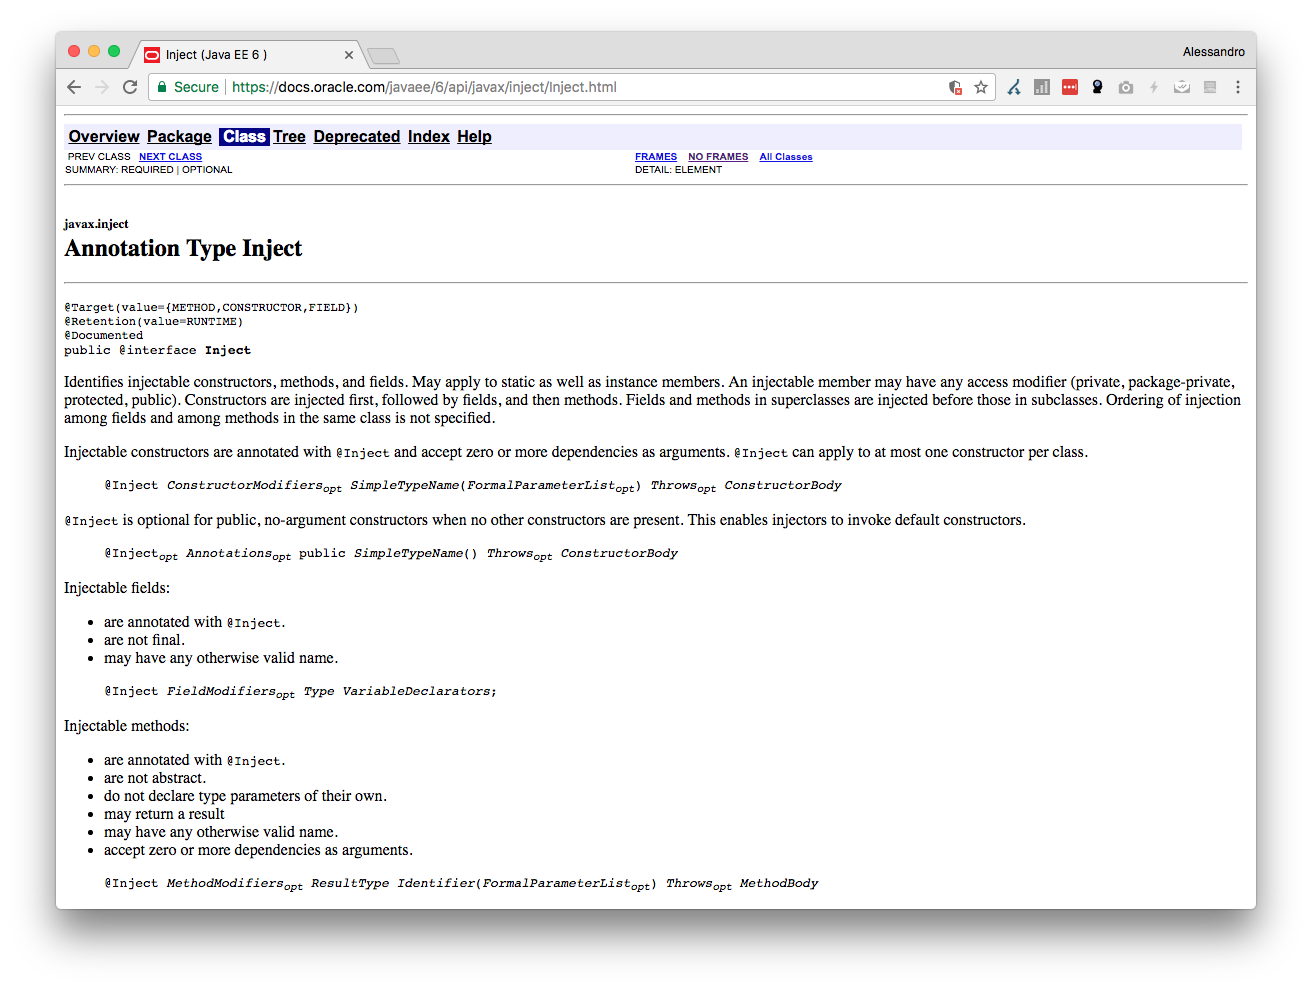
\includegraphics[width=.9\textwidth]{inject}
	\end{figure}
	\url{https://docs.oracle.com/javaee/6/api/javax/inject/Inject.html}
\end{frame}

\begin{frame}[fragile]
	Ingredients:%
	\footnote{Preparing the ground for dagger terminology, but here we are not using dagger yet}
	\begin{description}
		\item[modules]: it containes recipies (methods) to instantiate the dependencies 
		\item[injector/component]: wiring  and feed the target with the dependencies it needs 
	\end{description}
\end{frame}
\begin{frame}[fragile]
\begin{lstlisting}[language=Kotlin, basicstyle=\ttfamily]
// injector 
interface Component {
    fun inject(activity : MainActivity)
}

// provides the dependencies 
class Module {
    fun providePresenter(): Presenter {
        
    }
}
\end{lstlisting} 
\end{frame}
	\section{Dagger2}
	\section{Dagger2 Android }
	\section{Alternative patterns}
	\begin{frame}
		\begin{itemize}
			\item Cake pattern
			\item Reader monad 
			\item Implicits (Scala)
		\end{itemize}
	\end{frame}
\plain{Questions?}

%\begin{frame}[allowframebreaks] {References}
% \bibliography{demo}
% \bibliographystyle{abbrv}
%\end{frame}

\end{document}
